%MẪU LÀM CÂU HỎI TRẮC NGHIỆM THEO BẢNG
%Dùng với gói lệnh dethi.sty
%Dùng Vietex 2.8. với phông mã Unicode
%Người soạn : Nguyễn Hữu Điển, ĐHKHTN, ĐHQG HN
%Mail: huudien@vnu.edu.vn, CQ: (84 - 4) 557 2869
%NR: (84 - 4) 641 8848, DĐ: 0989061951
%Ngày 26/12/2009
%%%%%%%%%%%%%%%%%%%%%%%%%

\bangtracnghiem{bangtn:1}{
Trong phương án sau đây, 
phương án nào của hàm mũ tiếp cận với  $y = 0$ ?
}{%Phương án trả lời
\khong{$\displaystyle\lim_{x \to +\infty} \text{e}^x   =  + \infty$ }
\chon{$\displaystyle\lim_{x \to -\infty} \text{e}^x = 0$}
\khong{$\displaystyle\lim_{x \to +\infty} \dfrac{\text{e}^x}{x}  =   + \infty$ }
}%Hết một bài


\bangtracnghiem{bangtn:2}{
exp$(\ln x) = x$ pour tout $x$ appartenant à 
}{%Phương án trả lời
\chon{$\mathbf{R}$}
\khong{$\big]0~;~+ \infty\big[$}
\khong{$\big[0~;~+\infty\big[$}
}%Hết một bài


\bangtracnghiem{bangtn:3}{
Trong phương án sau đây, phương án nào của hàm mũ tiếp cận với  $y = 0$ ?
}{%Phương án trả lời
\khong{$\displaystyle\lim_{x \to +\infty} \text{e}^x   =  + \infty$}
\chon{$\displaystyle\lim_{x \to -\infty} \text{e}^x = 0$}
\khong{$\displaystyle\lim_{x \to +\infty} \dfrac{\text{e}^x}{x}  =   + \infty$}
}%Hết một bài

\bangtracnghiem{bangtn:4}{
exp$(\ln x) = x$ với mọi $x$ xác định 
}{%Phương án trả lời
\khong{$\mathbf{R}$}
\khong{$\big]0~;~+ \infty\big[$}
\chon{$\big[0~;~+\infty\big[$}
}%Hết một bài

\bangtracnghiem{bangtn:6}{
Trong phương án sau đây, phương án nào của hàm mũ tiếp cận với  $y = 0$ ?
}{%Phương án trả lời
\khong{$\displaystyle\lim_{x \to +\infty} \text{e}^x   =  + \infty$ }
\khong{$\displaystyle\lim_{x \to -\infty} \text{e}^x = 0$ }
\chon{$\displaystyle\lim_{x \to +\infty} \dfrac{\text{e}^x}{x}  =   + \infty$}
}%Hết một bài

\bangtracnghiem{bangtn:7}{
Với mọi số thực $x$, tập hợp $\dfrac{\text{e}^x - 1}{2}$
}{%Phương án trả lời
\khong{$\text{e}^x + 2\hskip12pt \text{bằng :}$  }
\chon{$-\dfrac{1}{2}$ }
\khong{$\dfrac{\text{e}^{-x} - 1}{\text{e}^{-x} + 2}$ }
\khong{$\dfrac{1 - \text{e}^{-x}}{1 + 2\text{e}^{-x}}$ }
}%Hết một bài

\bangtracnghiem{bangtn:8}{
Với mọi $x \in ]-\infty~;~2],~f’(x) \geqslant 0$.
}{%Phương án trả lời
\khong{ Sai }
\chon{ Đúng }
}%Hết một bài

\bangtracnghiem{bangtn:9}{
Hàm số $F$ có cực đại tại  $2$
}{%Phương án trả lời
\chon{ Đúng }
\khong{ Sai }
}%Hết một bài

\bangtracnghiem{bangtn:10}{
$\displaystyle\int_{0}^2 f’(x)\:\text{d}x = - 2$
}{%Phương án trả lời
\chon{ Đúng }
\khong{ Sai }
}%Hết một bài

\bangtracnghiem{bangtn:11}{
 Cho $f$ một hàm xác định và có đạo hàm trong khoảng%
$]-5~;~+\infty[$ trong bảng biến thiên:

% \input hinh1.tex
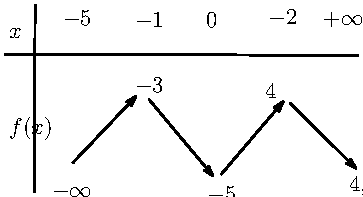
\includegraphics[scale =0.7]{hinh1}

Ký hiệu $\mathcal{C}$ tập hợ các hàm $f$.

Trên khoảng $]-5~;~+\infty[$, phương trình $f(x) = -2$ có
}{%Phương án trả lời
\khong{một nghiệm}
\chon{hai nghiệm}
\khong{bốn nghiệm}
}%Hết một bài



\bangtracnghiem{bangtn:5}{
Ma trận%
$M=\begin{pmatrix}
0 & 1 \\
1 & 1 \\
\end{pmatrix}$  là toàn phương với
}{%Phương án trả lời
\khong{$\begin{pmatrix}
0 & 1 \\
1 & 4 \\
\end{pmatrix}$}
\chon{$\begin{pmatrix}
1 & 2 \\
2 & 5 \\
\end{pmatrix}$}
 }%Hết một bài

